\begin{frame}
  \frametitle{Time-Dependent Multiphysics Simulations with the Hybrid Method}
  I investigated two transient scenarios based on actual MSRE experiments:
  \begin{block}{\textbf{MSRE Rod Drop Experiment}}
    \begin{itemize}
      \item Neutronic response of an initially critical, zero-power MSRE to a
        rod drop of Rod 1 \cite{prince_zero-power_1968}
      \item Corresponds to a reactivity withdrawal of -1500 pcm
      \item Requires delayed neutron precursor (DNP) modeling
    \end{itemize}
  \end{block}
  \begin{block}{\textbf{MSRE Reactivity Insertion Experiment}}
    \begin{itemize}
      \item Coupled power response of the MSRE initially at 1 MW to a rod
        withdrawal \cite{engel_zero-power_1972}
      \item Reactivity insertion of 24.8 pcm
      \item MSRE fueled with $^{233}$U
      \item Requires DNP and temperature advection-diffusion modeling
    \end{itemize}
  \end{block}
\end{frame}

\begin{frame}
  \frametitle{MSRE Rod Drop Experiment}
  \textbf{Rod Height}
  \begin{figure}[htb!]
    \centering
    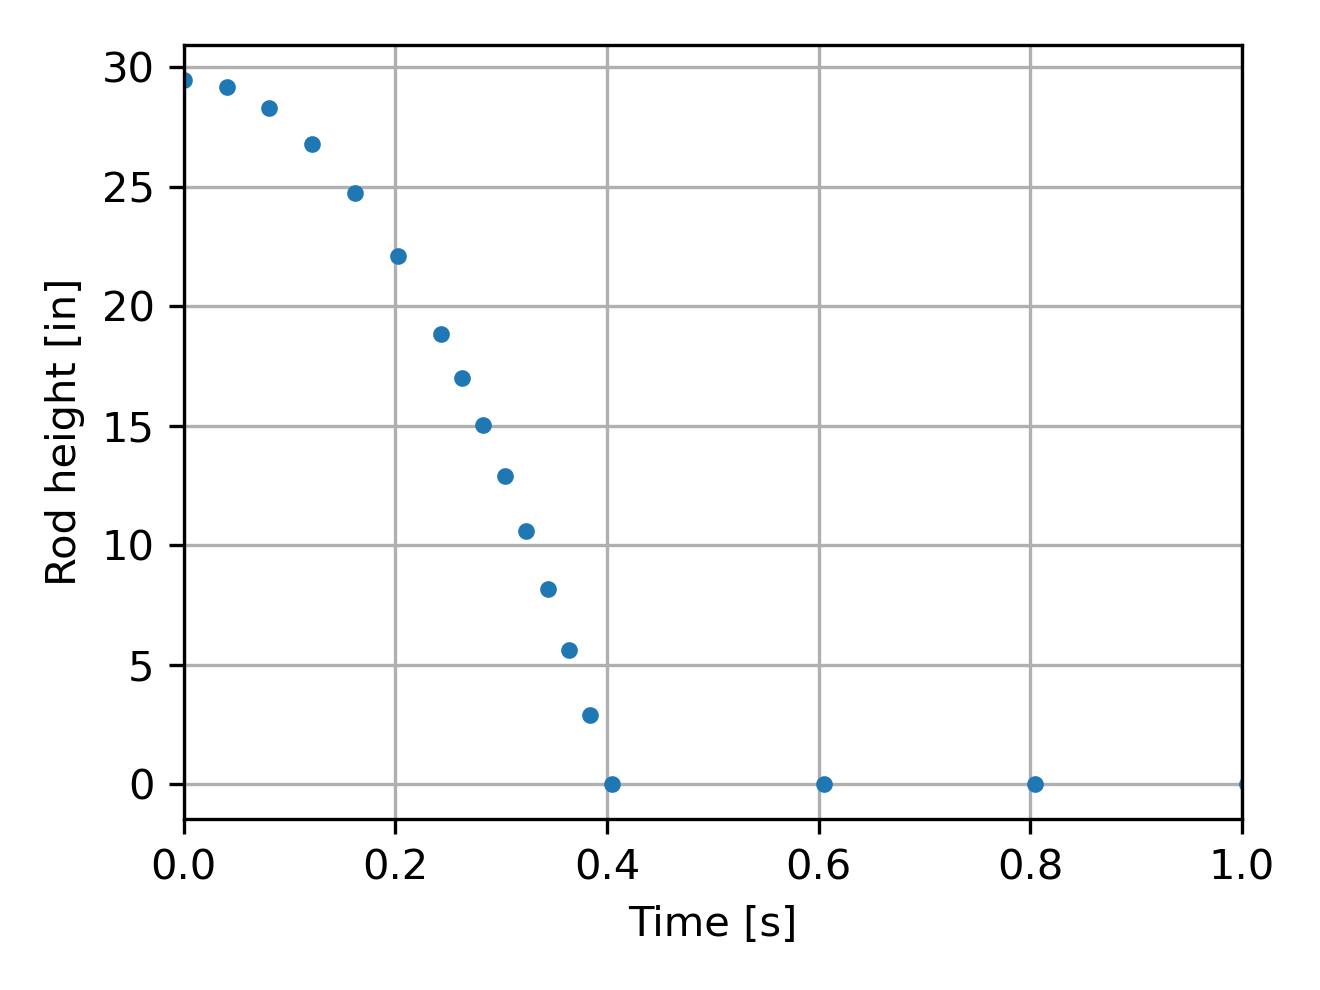
\includegraphics[width=0.7\columnwidth]{rod-height}
    \caption{Evolution of rod height evaluated at each timestep within the first second of the rod
    drop simulation. The rod reaches its fully inserted height at $t=0.4046$ s.}
    \label{fig:rod-height}
  \end{figure}
\end{frame}

\begin{frame}
  \frametitle{MSRE Rod Drop Experiment}
  \textbf{Nested Coupling Iteration Structure for the Rod Drop Simulation}
  \begin{figure}[t]
    \tikzstyle{every node}=[font=\small]
    \centering
    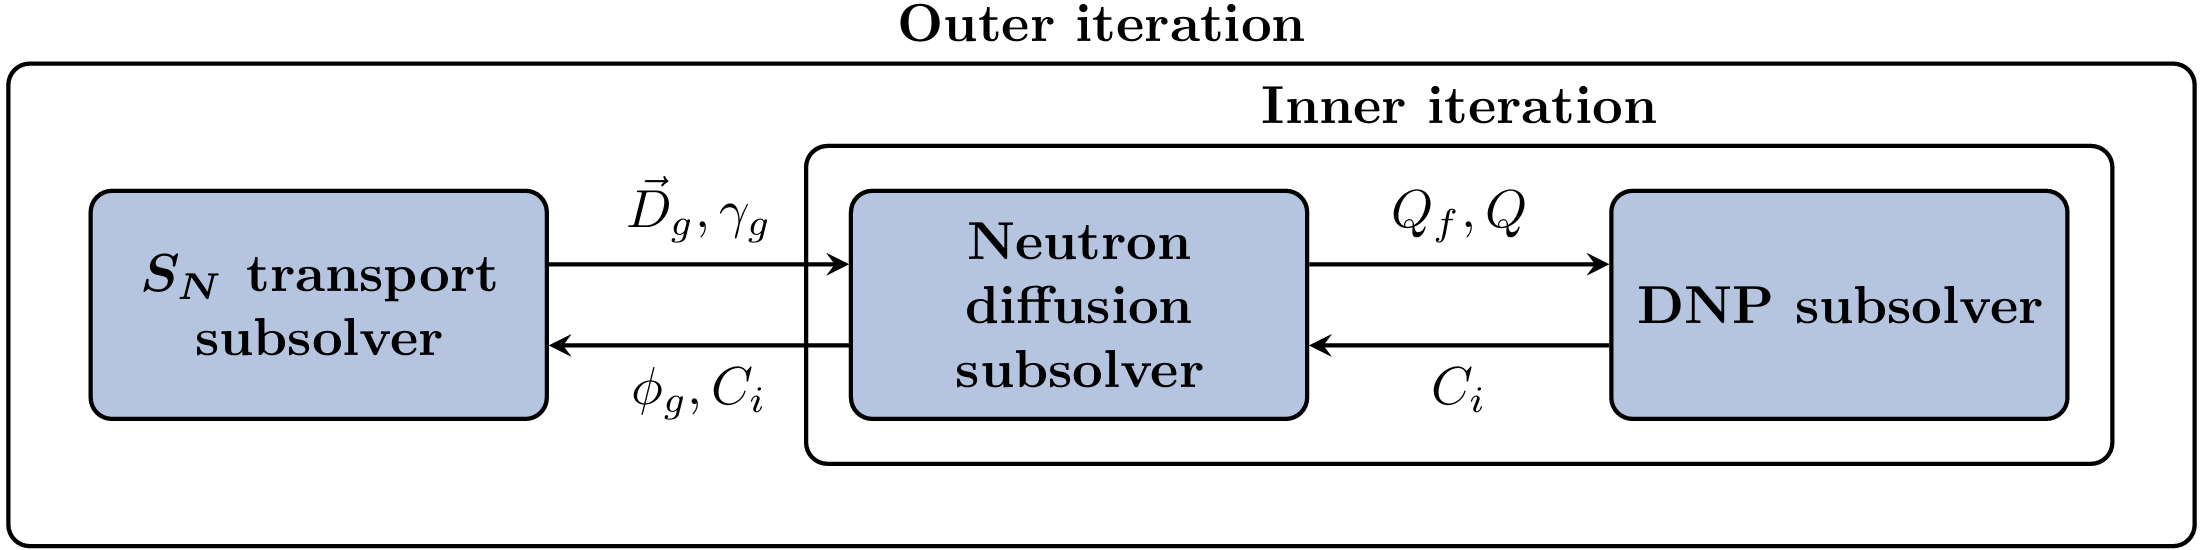
\includegraphics[width=\columnwidth]{images/nest-1}
    \caption{The nested iteration structure coupling the $S_N$, neutron diffusion, and \gls{DNP}
    solvers for the rod drop simulation using the hybrid $S_N$-diffusion method.}
    \label{fig:rod-drop-coupling}
  \end{figure}
\end{frame}

\begin{frame}
  \frametitle{MSRE Rod Drop Experiment}
  \textbf{Integral Neutron Count Following Rod Drop}
  \begin{figure}[t]
    \centering
    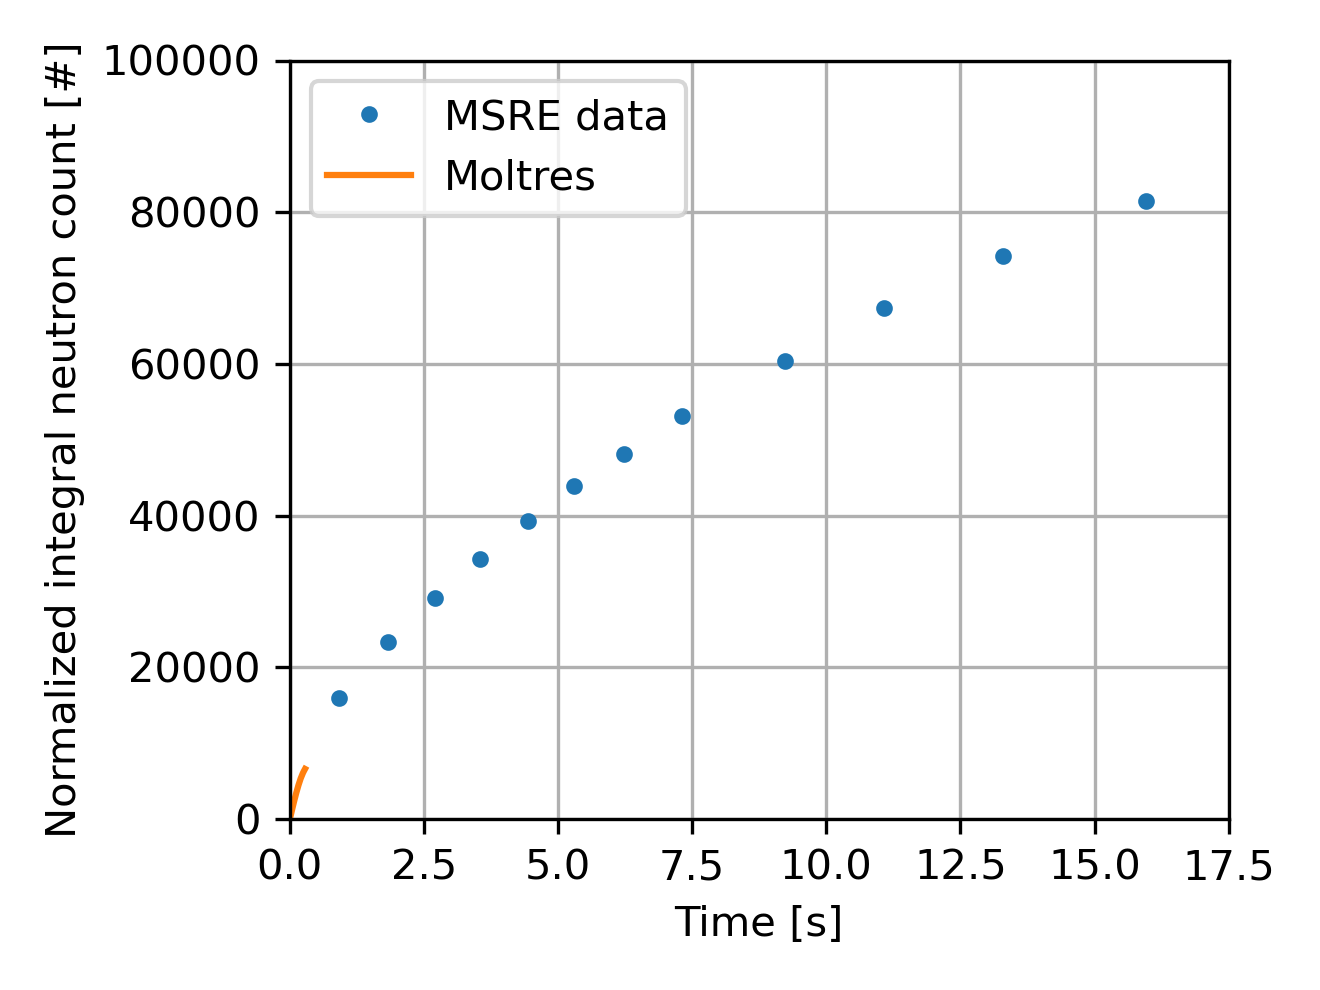
\includegraphics[width=0.55\columnwidth]{integral-count}
    \caption{Integral neutron count during the rod drop experiment from \gls{MSRE} experimental data
    and hybrid method numerical results.}
    \label{fig:integral-count}
  \end{figure}
  \begin{itemize}
    \item Moltres underpredicted the integral neutron count rate by approximately 20 \%.
    \item Potential sources of error
    \begin{itemize}
      \item Uncertainty in the initial neutron count rate
      \item Miscalculation of -1500 pcm reactivity withdrawal
    \end{itemize}
  \end{itemize}
\end{frame}

\begin{frame}
  \frametitle{MSRE Reactivity Insertion Experiment}
  \textbf{Nested Coupling Iteration Structure for the Reactivity Insertion Simulation}
  \begin{figure}[t]
    \centering
    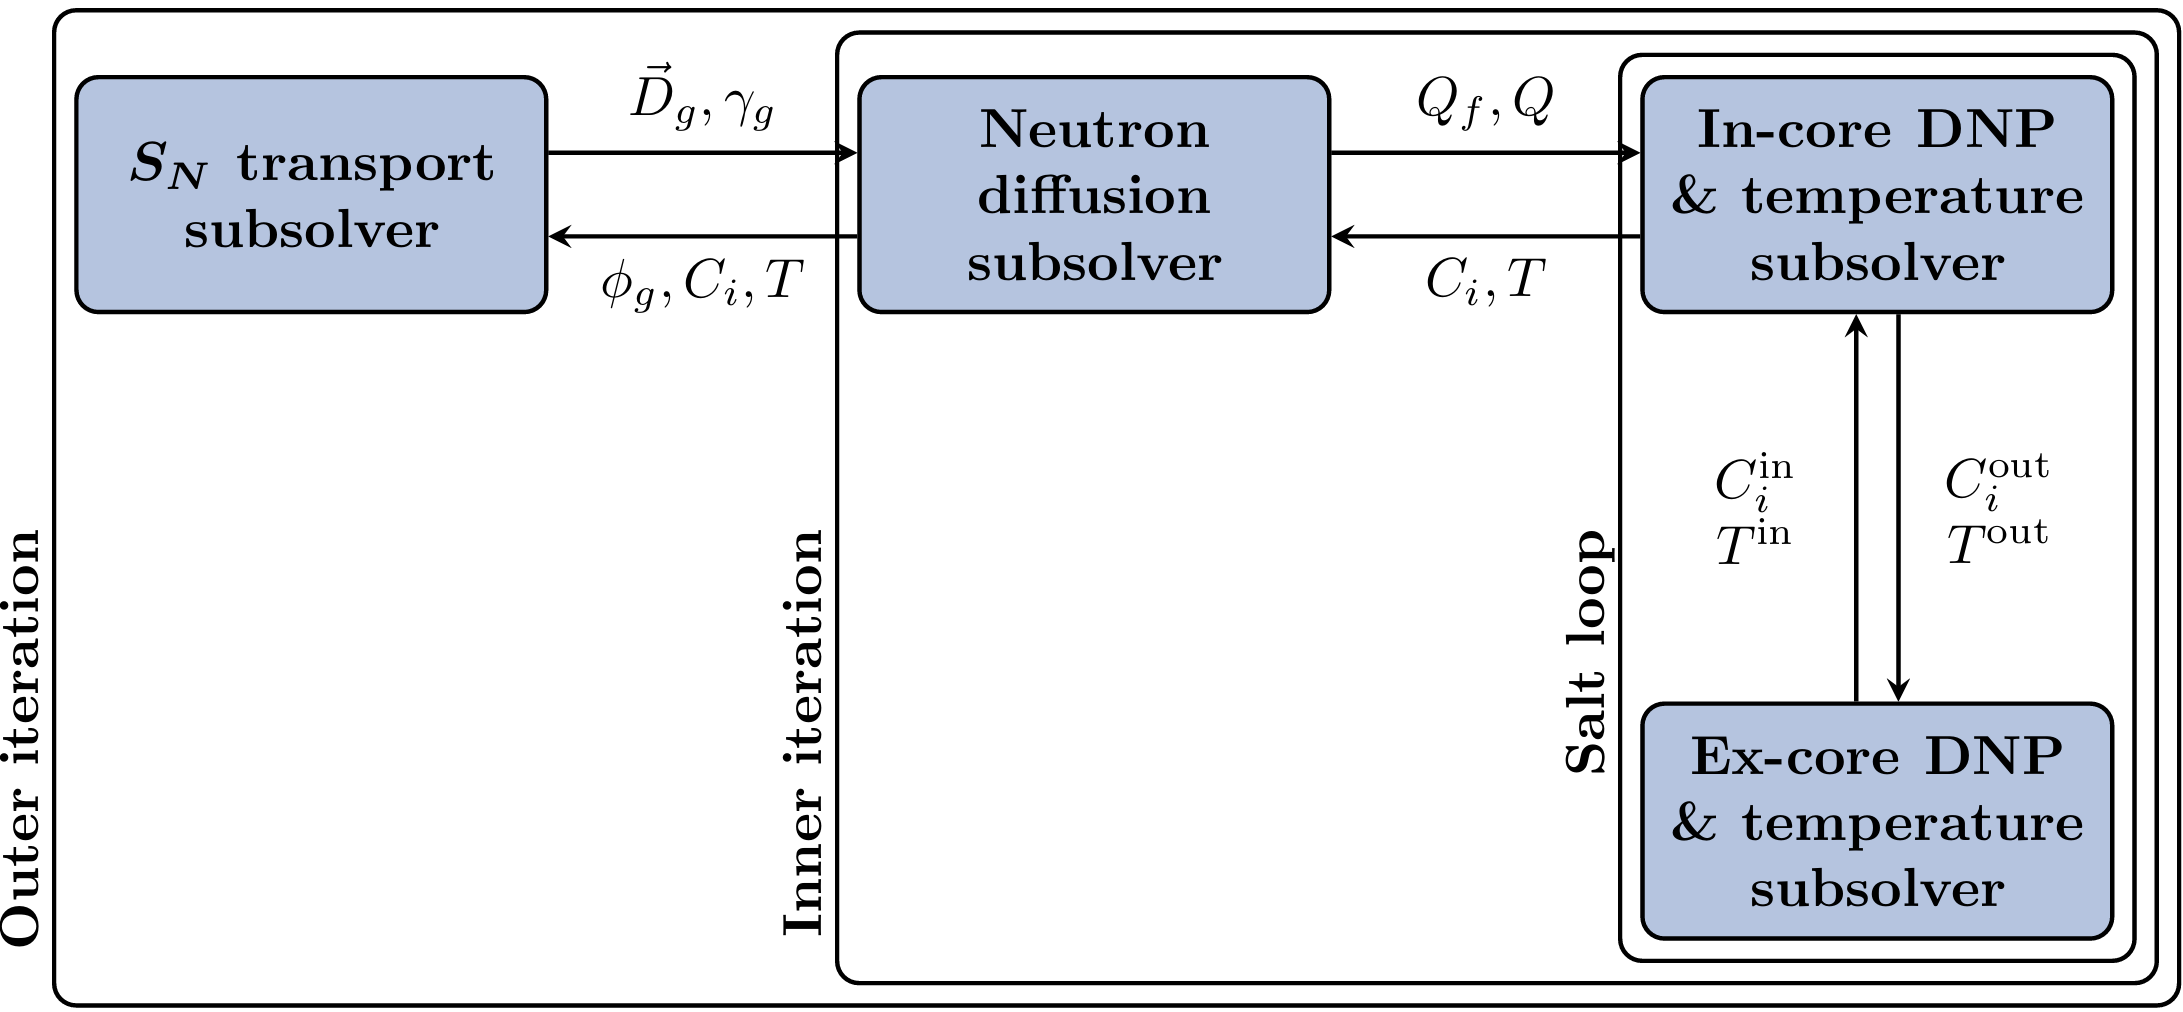
\includegraphics[width=\columnwidth]{images/nest-2}
    \caption{The nested iteration structure coupling the $S_N$, neutron diffusion,
    in-core \gls{DNP}-temperature, and ex-core
    solvers for the reactivity insertion simulation using the hybrid $S_N$-diffusion method.}
    \label{fig:insertion-coupling}
  \end{figure}
\end{frame}
